\section{Excercise 10}
Cho mạch sau. Tìm điện áp V. Bạn có thể làm điều này bằng mọi cách nhưng hãy nhớ để giải thích nó một cách chi tiết. Sau đó mô phỏng mạch để kiểm tra kết quả.\\
\begin{figure}[!htbp]
    \centering
    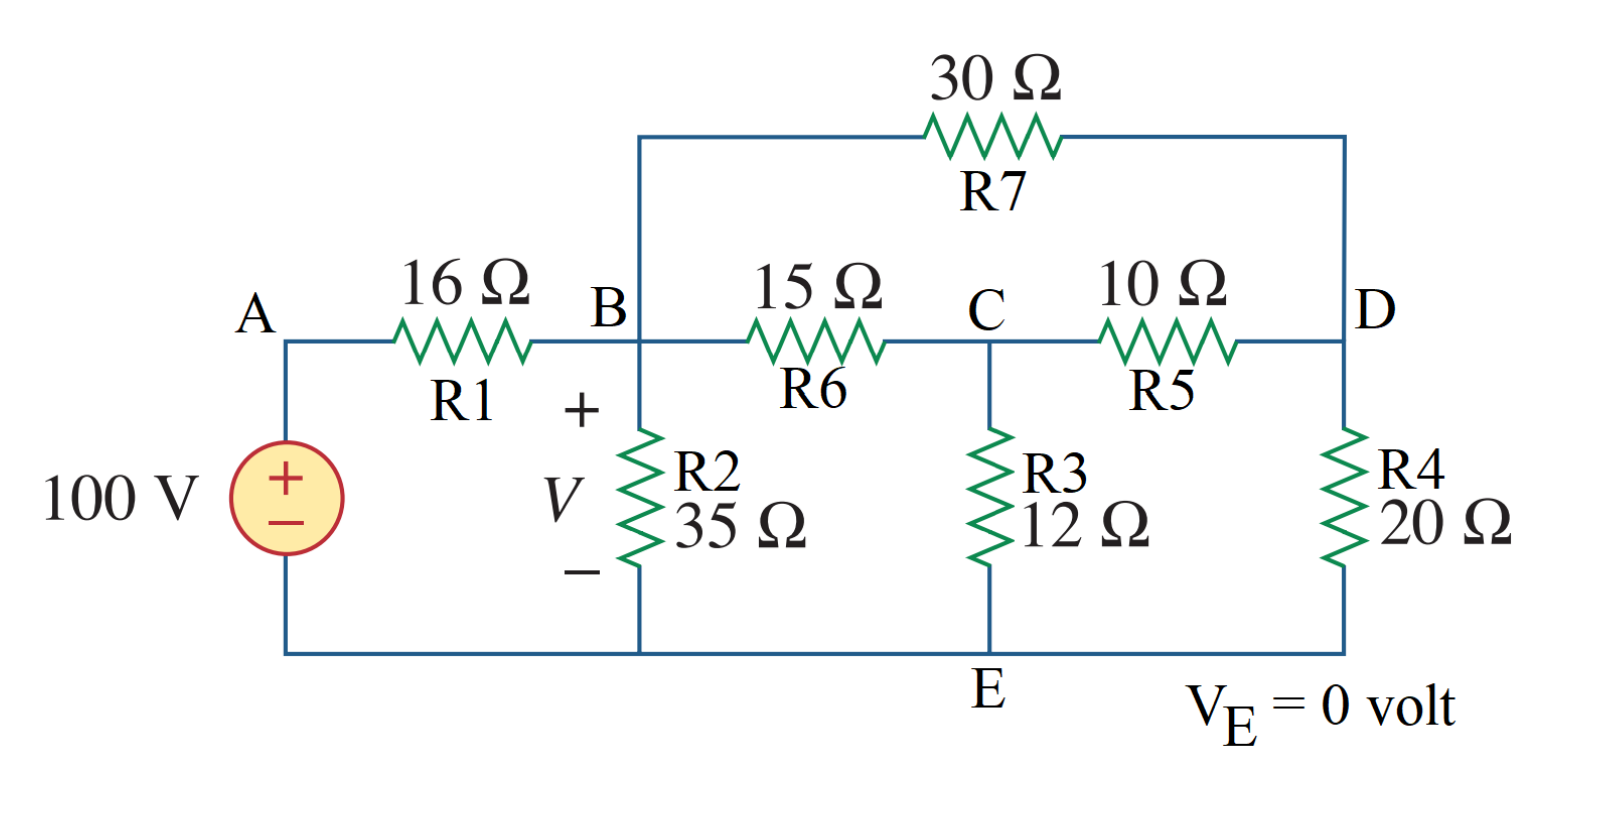
\includegraphics[width=0.7\textwidth]{graphics/ex10/f1.png}
    \caption{Tìm điện áp V}
\end{figure}
\textbf{Trả lời}
\subsection{Tính toán}
\begin{itemize}
    \item Biến đổi mạch về mạch đơn giản để tìm điện trở tương đương\\
    \begin{figure}[!htbp]
        \centering
        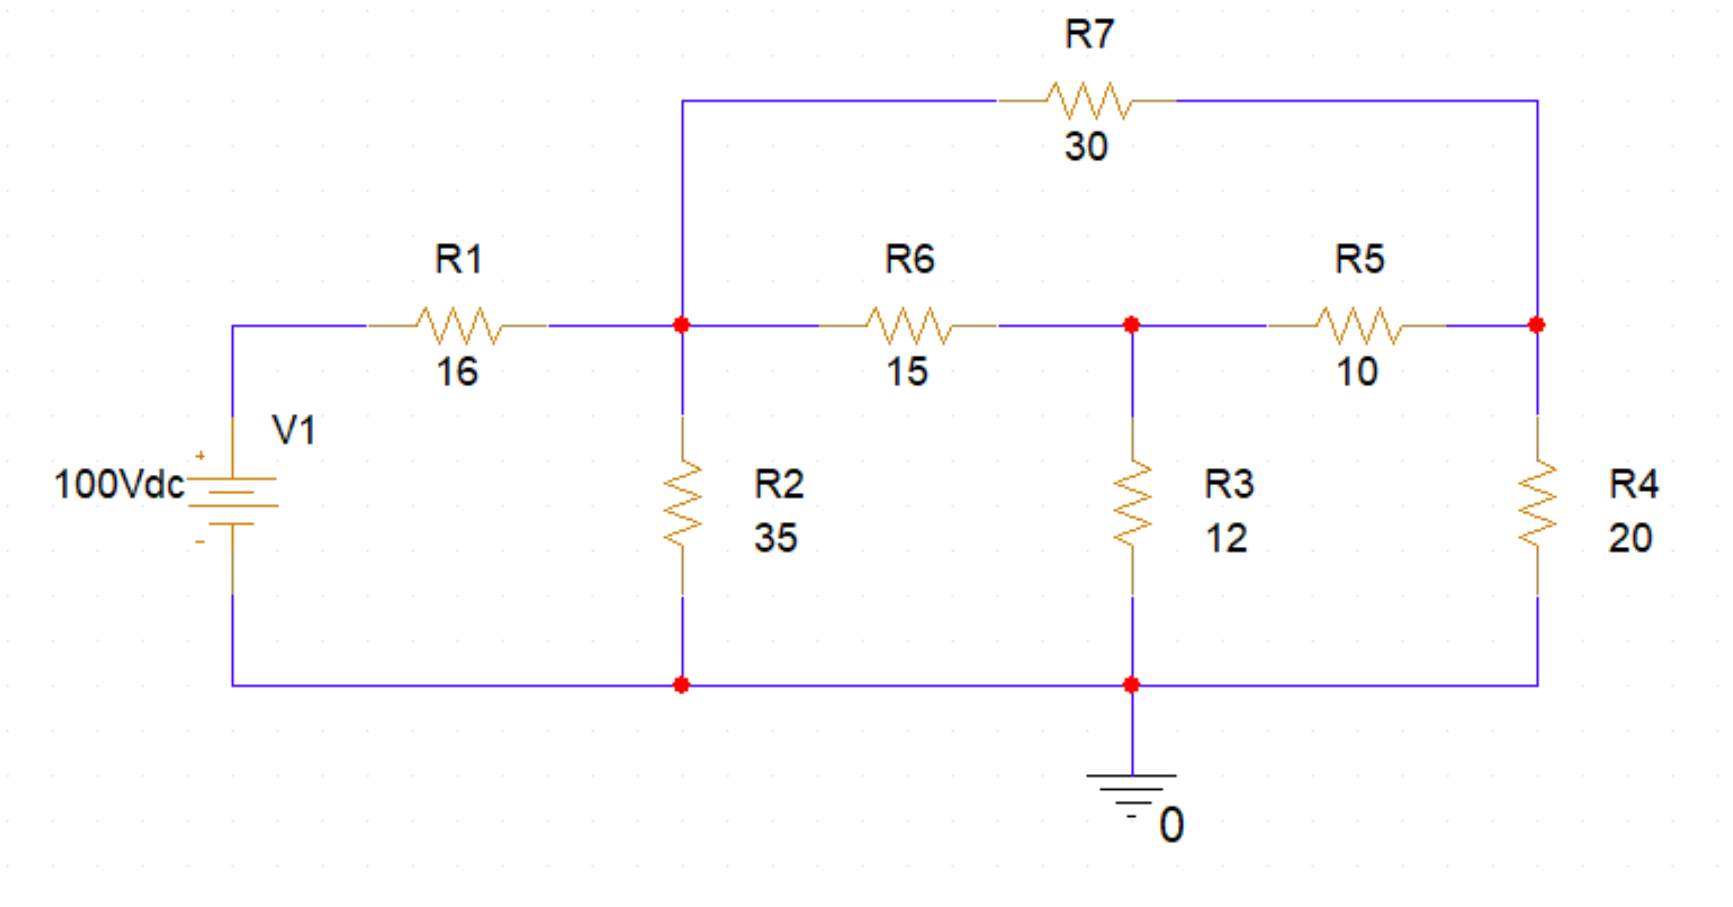
\includegraphics[width=0.8\textwidth]{graphics/ex10/f2.png}
        \caption{Mạch ban đầu}
        \end{figure}\\
        \begin{figure}[!htbp]
            \centering
            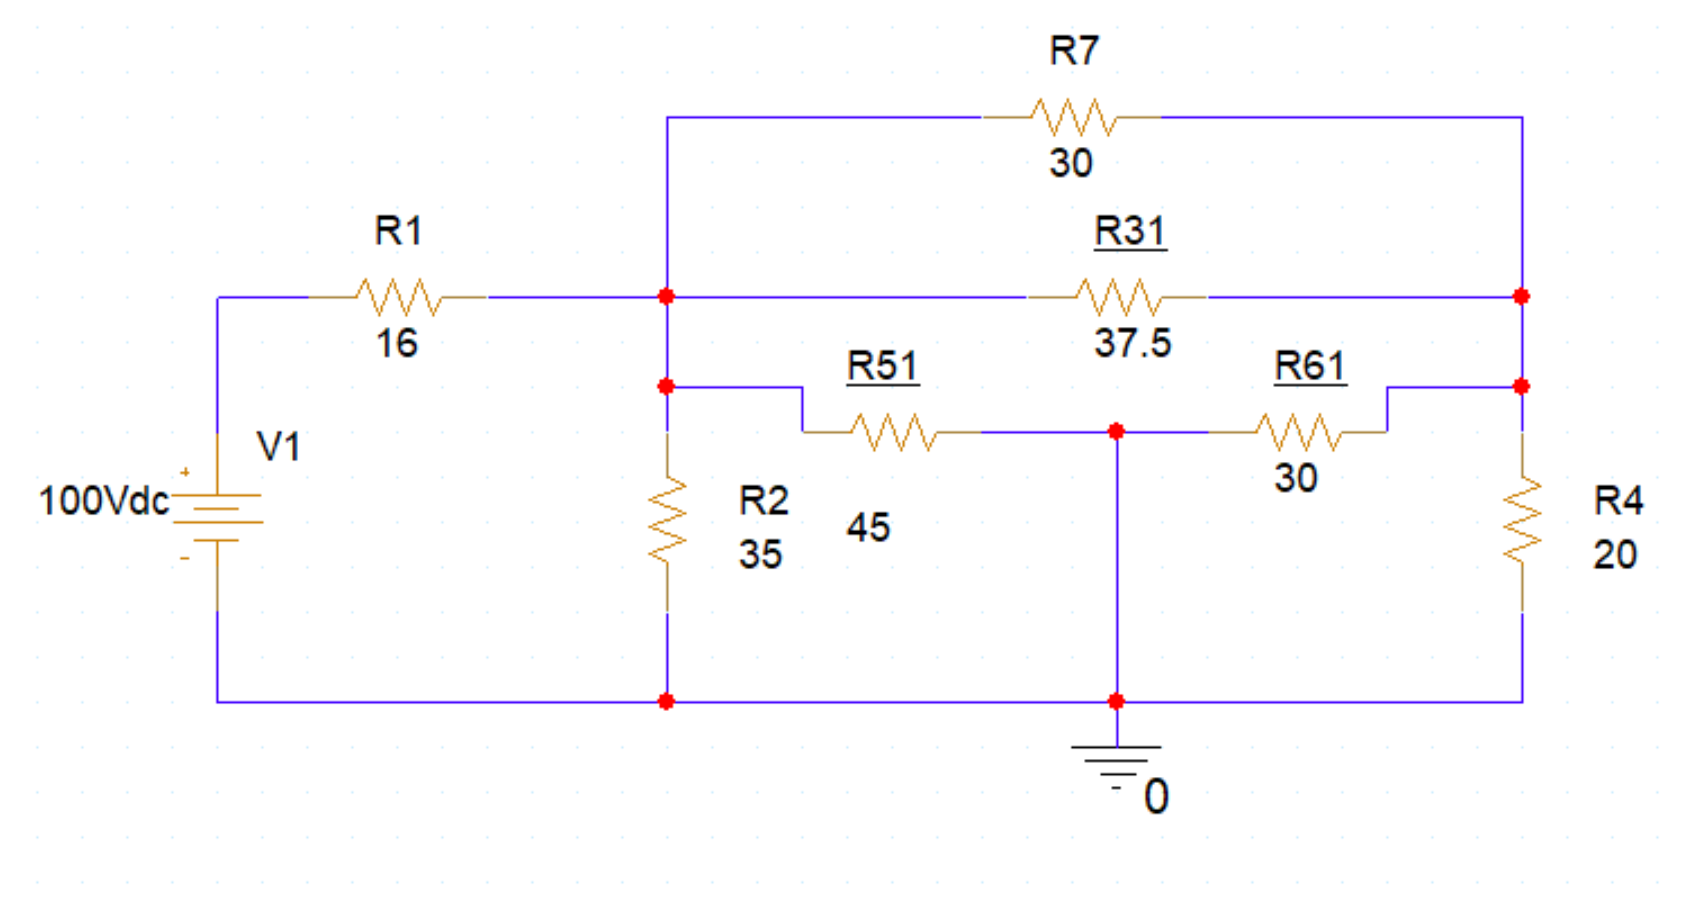
\includegraphics[width=0.8\textwidth]{graphics/ex10/f3.png}
            \caption{Dùng biến đổi wye-delta chuyển mạch wye \(R_3-R_5-R_6\) thành mạch delta \(R_{31}-R_{51}-R_{61}\)}
            \end{figure}\\
    Tính toán các giá trị:
    \begin{align*}
        R_{31} = \dfrac{R_3.R_5 + R_5.R_6 + R_6.R_3}{R_3} = 37,5 (\Omega).\\
        R_{51} = \dfrac{R_3.R_5 + R_5.R_6 + R_6.R_3}{R_5} = 45 (\Omega).\\
        R_{61} = \dfrac{R_3.R_5 + R_5.R_6 + R_6.R_3}{R_3} = 30 (\Omega).\\
    \end{align*}
    \begin{figure}[!htbp]
        \centering
        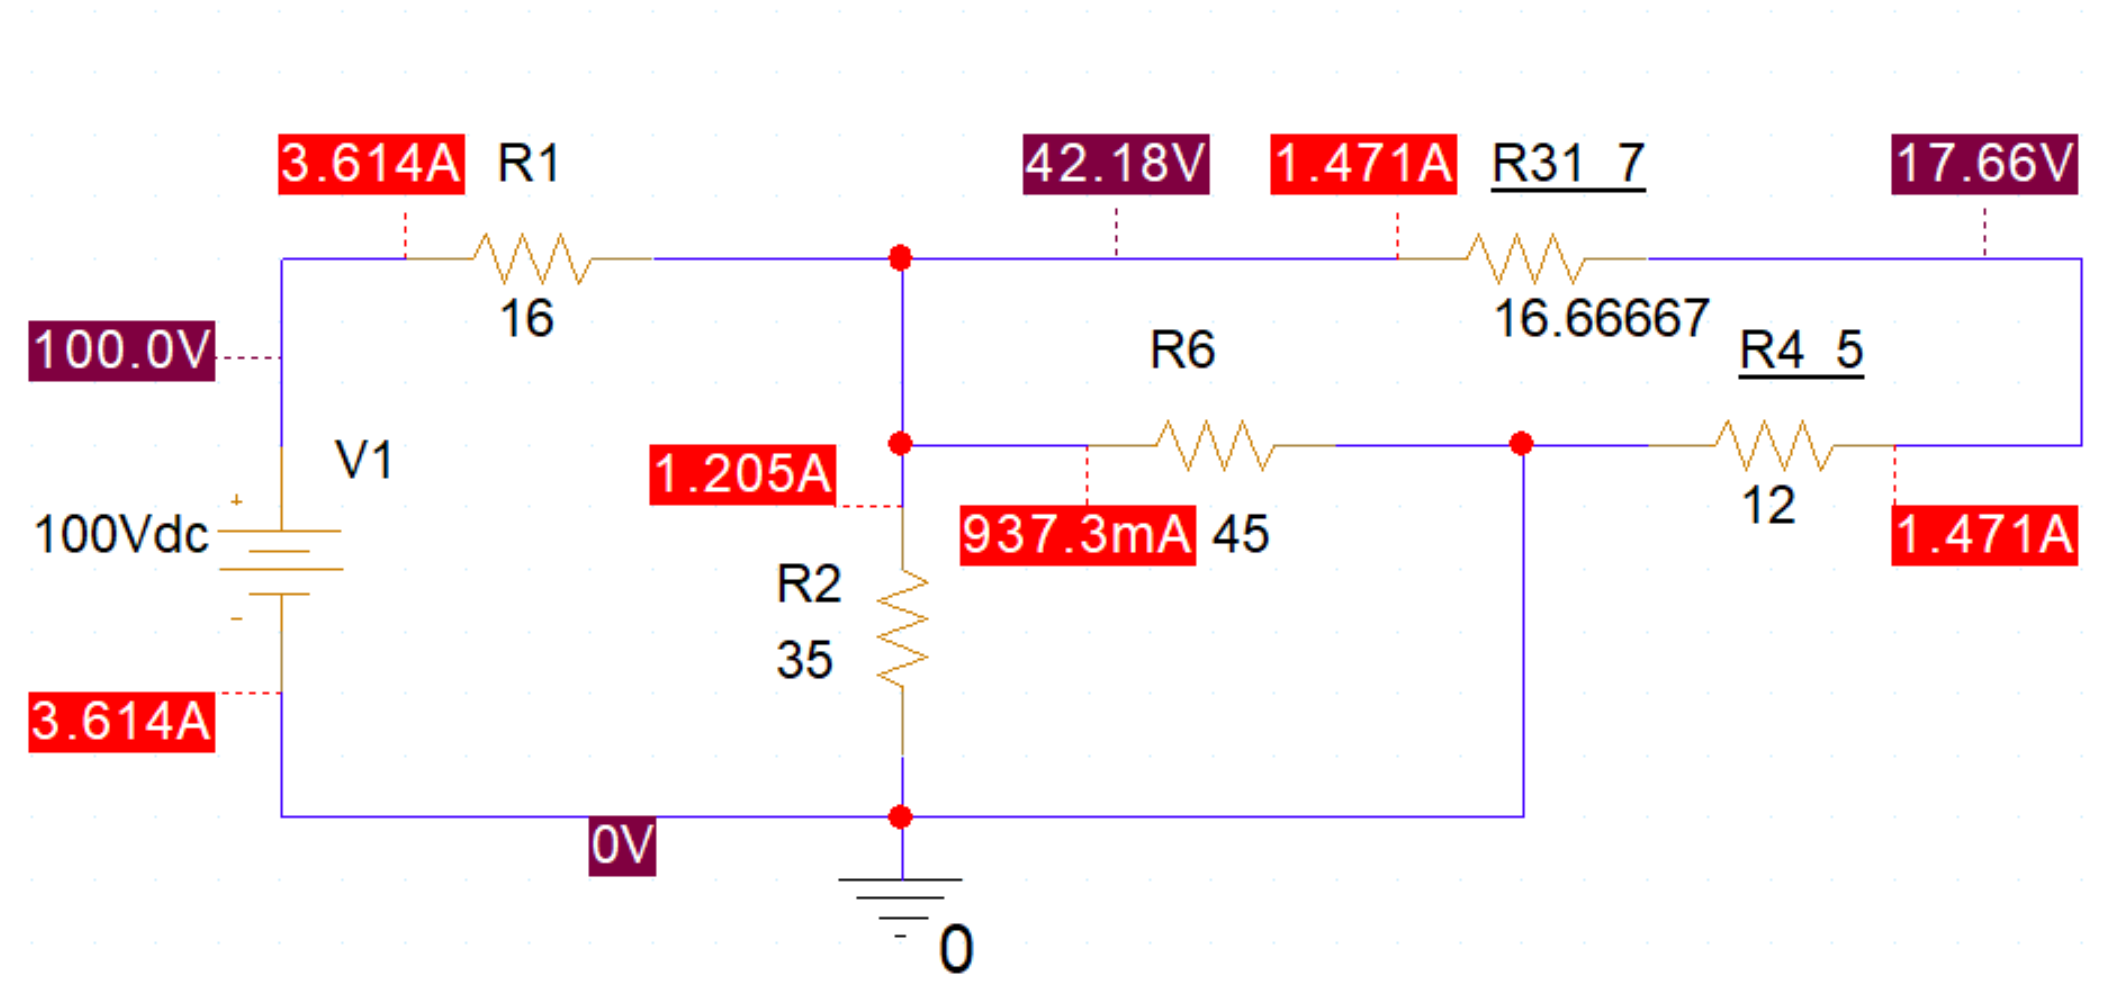
\includegraphics[width=0.8\textwidth]{graphics/ex10/f8.png}
        \caption{Biến đổi \(R_{61} // R_4\) thành \(R_{4\_61}\), \(R_7 // R_{31}\) thành \(R_{31\_7}\)}
        \end{figure}\\
    Tính toán các giá trị:
    \begin{align*}
        R_{31} // R_7 \rightarrow \dfrac{1}{R_{31\_7}} = \dfrac{1}{R_{31}} + \dfrac{1}{R_7} \rightarrow R_{31\_7} = 16,66667 (\Omega).\\
        R_{4} // R_{61} \rightarrow \dfrac{1}{R_{4\_61}} = \dfrac{1}{R_{61}} + \dfrac{1}{R_4} \rightarrow R_{4\_61} = 12 (\Omega).\\
    \end{align*}
    \begin{figure}[!htbp]
        \centering
        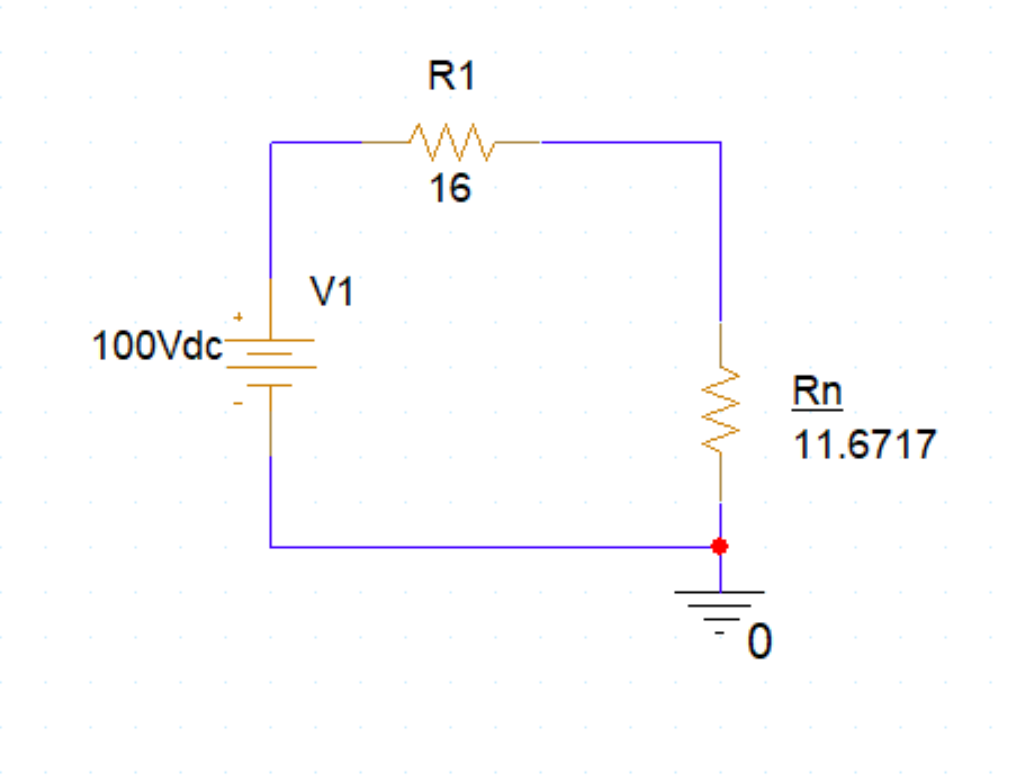
\includegraphics[width=0.8\textwidth]{graphics/ex10/f5.png}
        \caption{Biến đổi \((R_{31\_7} nt R_{4\_61})//R_{51}//R_2\) thành \(R_{n}\)}
        \end{figure}\\
        Tính toán các giá trị:
        \begin{align*}
            (R_{31\_7} nt R_{4\_61})//R_{51}//R_2 \rightarrow \dfrac{1}{R_n} = \dfrac{1}{R_{31\_7} + R_{4\_61}} + \dfrac{1}{R_{51}} + \dfrac{1}{R_2} \rightarrow R_n = 11,6717 (\Omega)
        \end{align*}
        
        Vậy điện trở tương đương \(R = R_1 + R_n = 27,6717 (\Omega)\).
    \item Theo định luật Ohm, \(I = \dfrac{V_1}{R} = \dfrac{100}{27,6717} = 3,614 (A)\)
    \pagebreak
    \item {Áp dụng định luật Kirchhoff's Voltage(KVL) cho vòng:
    \begin{figure}[!htbp]
        \centering
        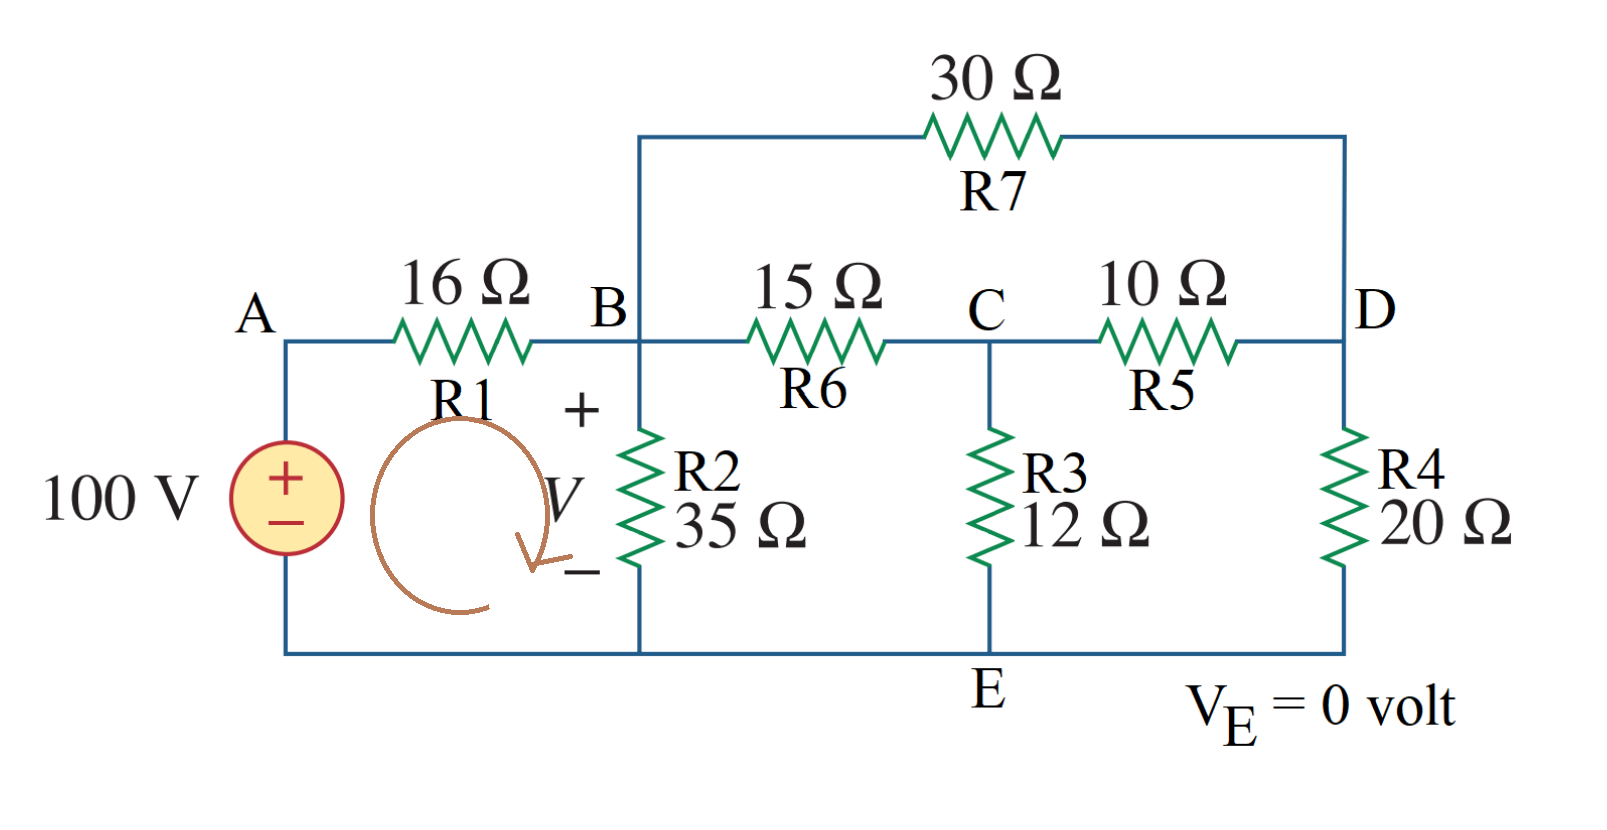
\includegraphics[width=0.8\textwidth]{graphics/ex10/f10.png}
        \end{figure}\\
        Ta có: \(I.R_1 + V - 100 = 0 \rightarrow 3,614.16 + V -100 = 0 \rightarrow V = 42,179 (V)\)}
\end{itemize}
\subsection{Mô phỏng}
\begin{figure}[!htbp]
    \centering
    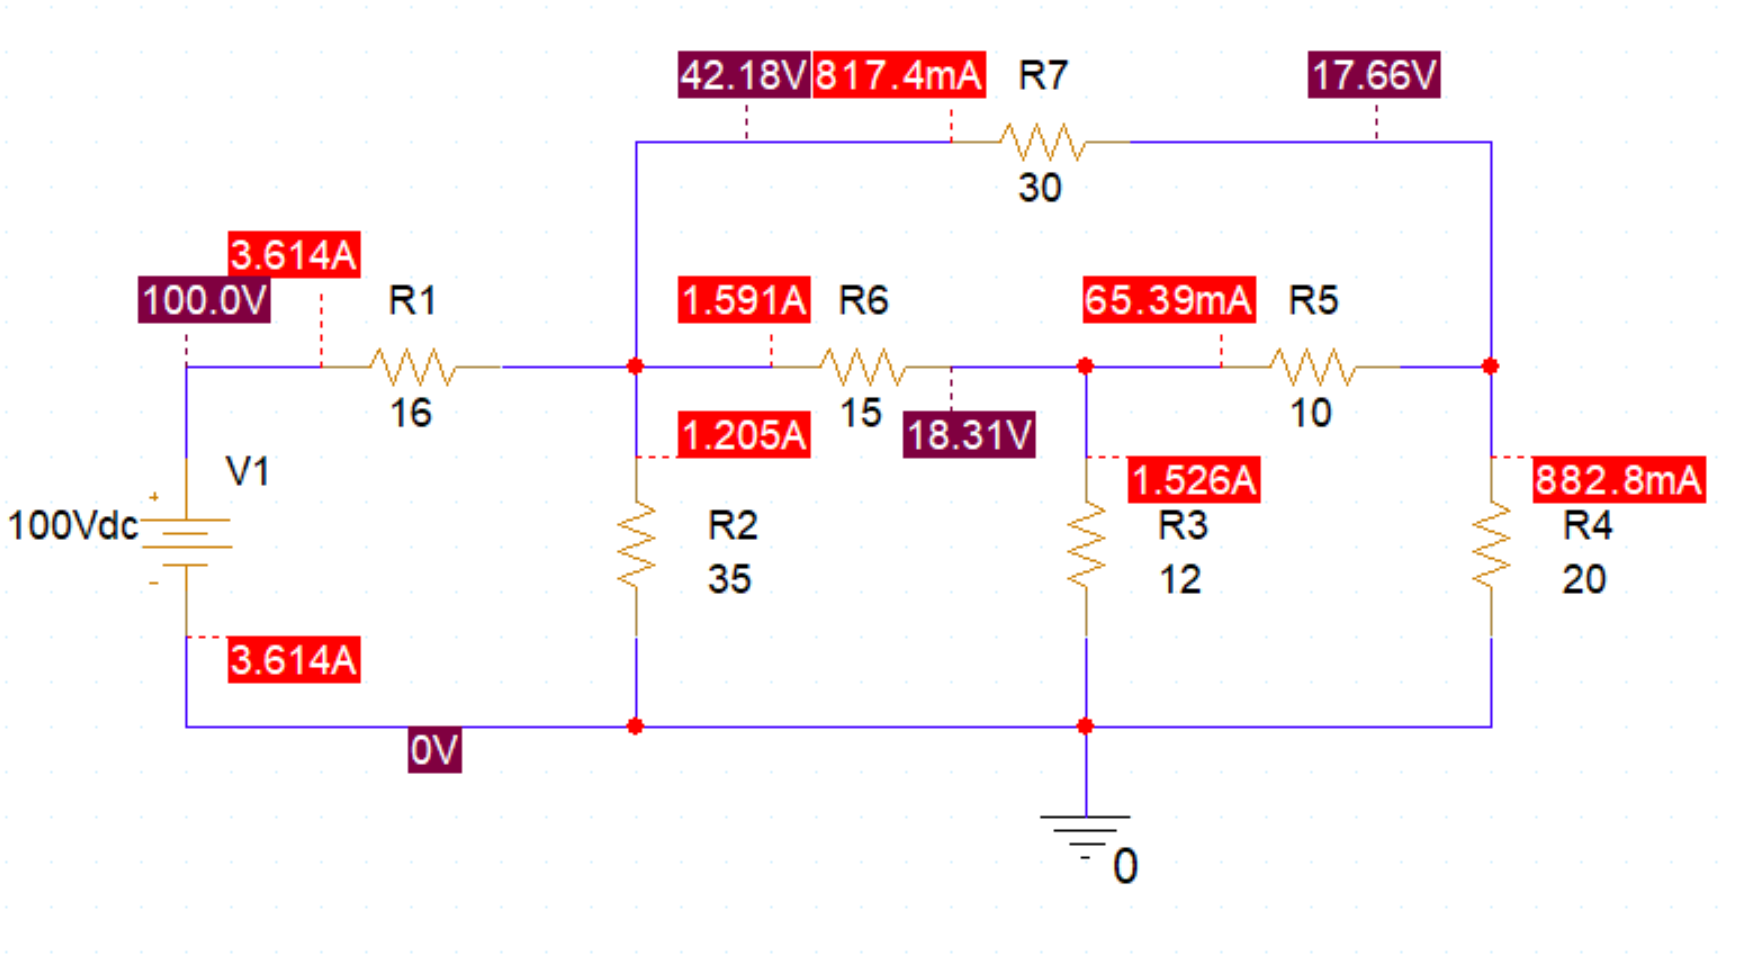
\includegraphics[width=0.9\textwidth]{graphics/ex10/f6.png}
    \caption{Mạch ban đầu}
\end{figure}
    \begin{figure}[!htbp]
        \centering
        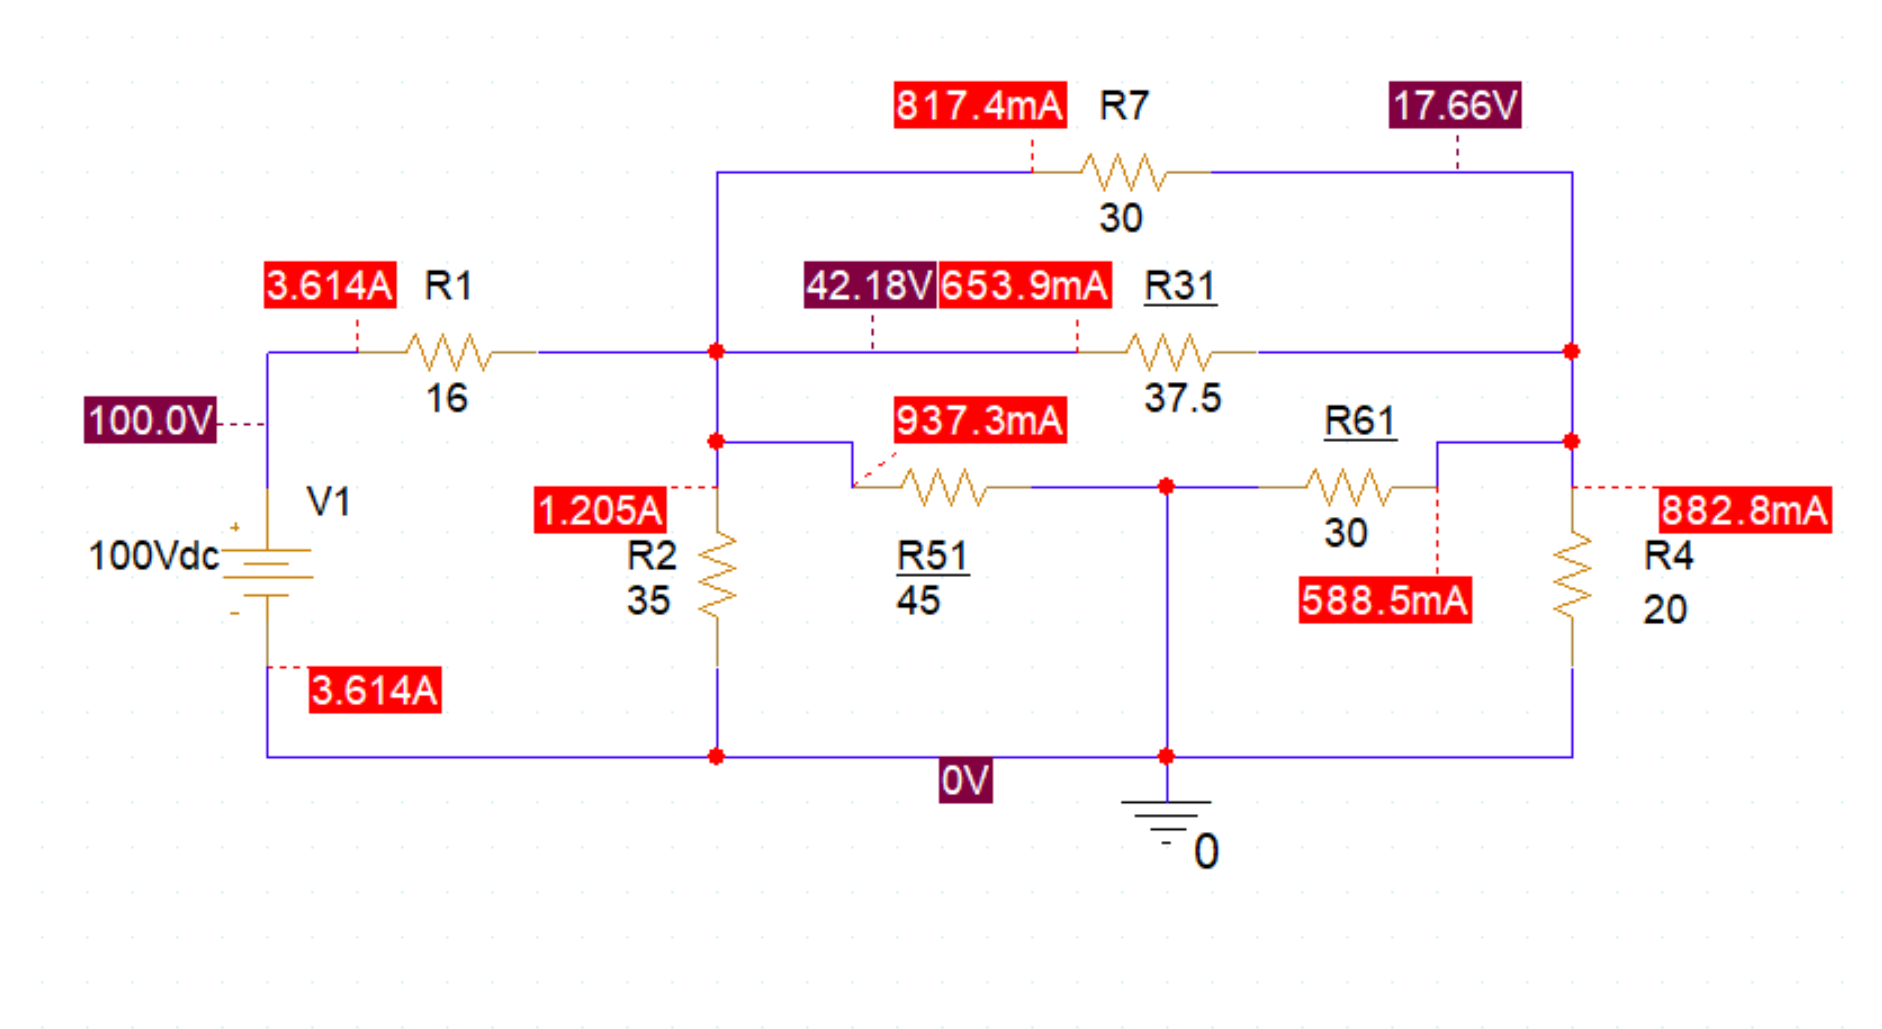
\includegraphics[width=0.9\textwidth]{graphics/ex10/f7.png}
        \caption{Mạch tương đương 1}
    \end{figure}

    \begin{figure}[!htbp]
            \centering
            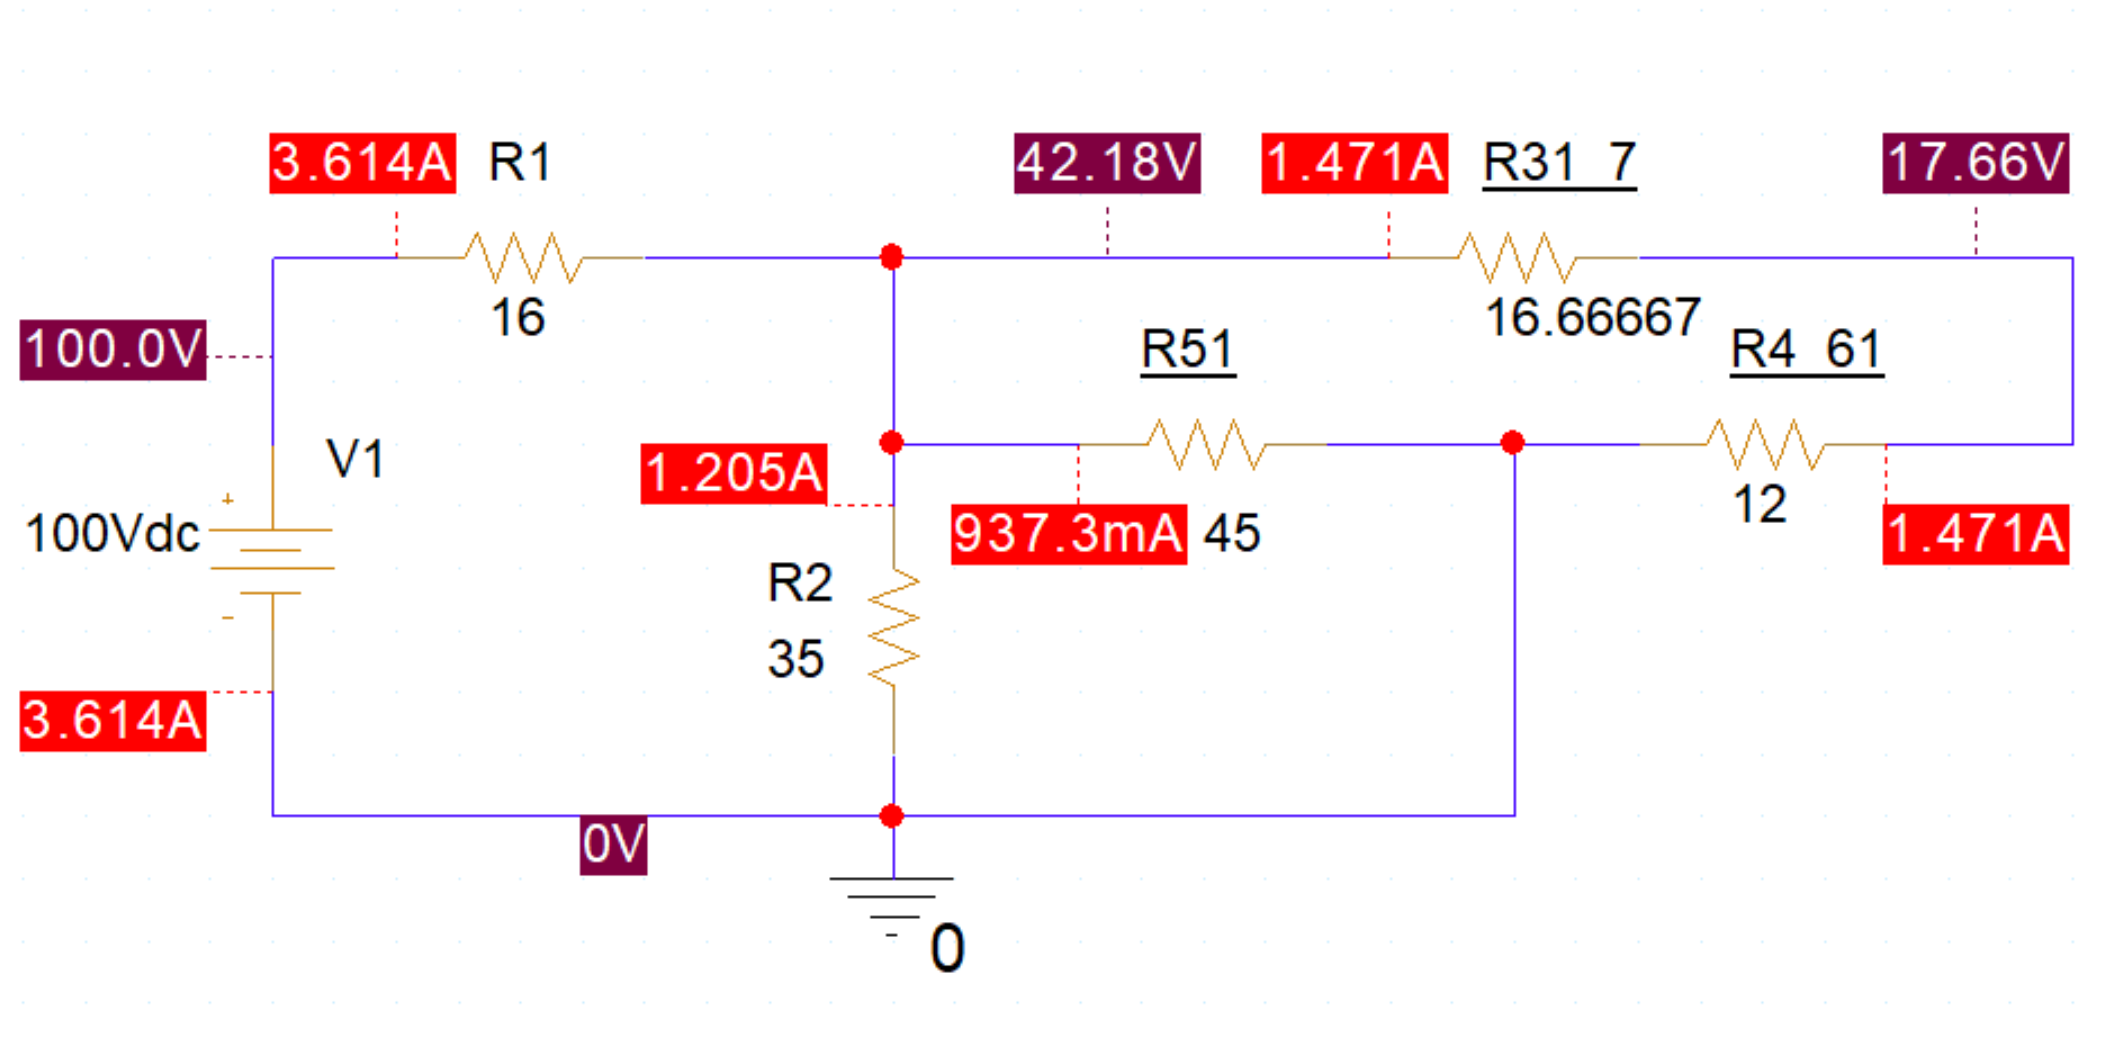
\includegraphics[width=0.9\textwidth]{graphics/ex10/f4.png}
            \caption{Mạch tương đương 2}
    \end{figure}

    \begin{figure}[!htbp]
                \centering
                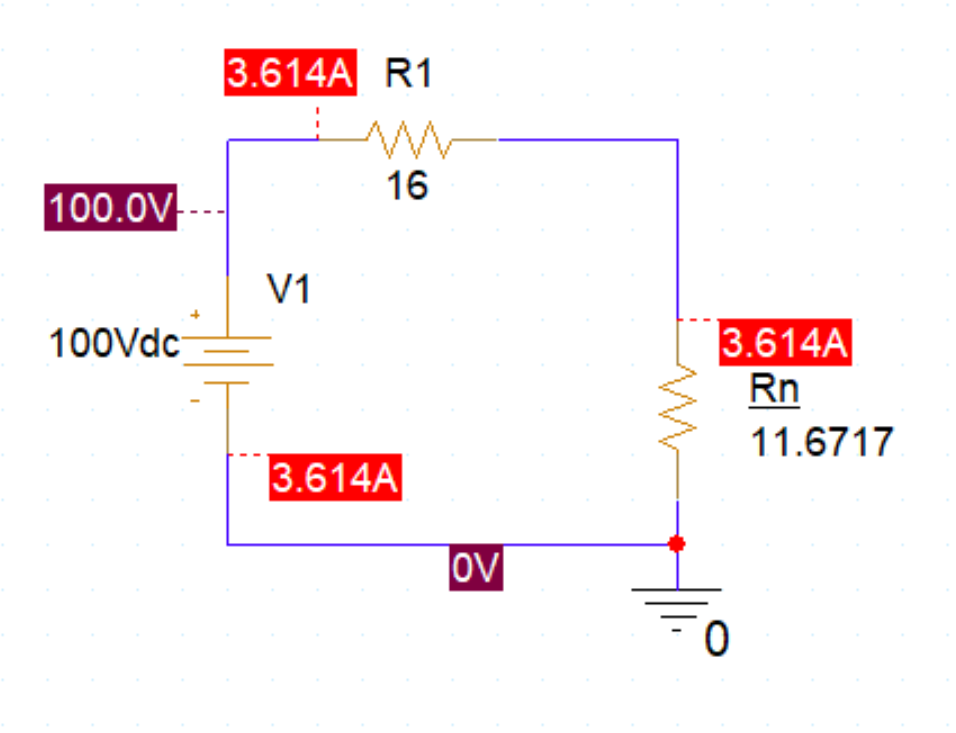
\includegraphics[width=0.7\textwidth]{graphics/ex10/f9.png}
                \caption{Mạch tương đương 3}
    \end{figure}
